% Metódy inžinierskej práce

\documentclass[10pt,twoside,slovak,a4paper]{article}


\usepackage[slovak]{babel}
%\usepackage[T1]{fontenc}
\usepackage[IL2]{fontenc} % lepšia sadzba písmena Ľ než v T1
\usepackage[utf8]{inputenc}
\usepackage{graphicx}
\usepackage{url} 
\usepackage{hyperref} 
\usepackage{}
%\usepackage{times}

\pagestyle{headings}

\title{Spiral model a jeho použitie pri modelovaní softvéru\thanks{Semestrálny projekt v predmete Metódy inžinierskej práce, ak. rok 2021/22, vedenie: Ing. Vladislav Mlynarovič, PhD.}} 

\author{Tomáš Andel\\[2pt]
	{\small Slovenská technická univerzita v Bratislave}\\
	{\small Fakulta informatiky a informačných technológií}\\
	{\small \texttt{xandelt1@stuba.sk}}
	}

\date{\small 30. september 2021}



\begin{document}

\maketitle

\begin{abstract}
Spiral model je metóda na vývoj softvéru. Vývoj pomocou tohto modelu sa vyznačuje tým, že kladie dôraz na redukciu riskov. Článok predstaví vývoj softvéru, niektoré tradičné modely, ich problémy a ako ich Spiral model rieši. Analyzuje postup vývoja pomocou Spiral modelu, porovná jeho výhody a nevýhody a predstaví ako vznikal a ako sa vyvíjal. Preskúma aké spôsoby modelovania sa využívajú pri vývoji touto metódou. Pozrie sa na rôzne možnosti jeho využitia a kde konkrétne sa používa. Predstaví novinky v tejto oblasti ako napríklad aké sú iné modely, ktoré sú založené na Spiral modeli alebo aké kombinácie Spiral modelu a iných modelov sa dnes využívajú na optimalizáciu vývoja softvéru.
\end{abstract}

\section{Úvod}

Vývoj softvéru je zložitý proces. Tvorba nápadu, určenie požiadaviek, dizajn, implementácia, testovanie, údržba - tieto všetky a ďalšie procesy nastávajú pri vývoji softvéru, bez jasného plánu môže byť vývoj zdĺhavý a drahý. Už od možnosti vývoja prvého softvéru ľudia hľadajú modely, podľa ktorých budú pracovať, a ktoré im umožnia efektívne vyvíjať komplexné softvéry.

Existuje množstvo vývojových modelov, niektoré sú vhodnejšie na menšie projekty, pričom sú nepoužiteľné vo veľkých, kde by vývoj postupoval neefektívnym spôsobom. Iné sú zasa vhodnejšie na veľké projekty, ale pri malých projektoch by bolo ich použitie zbytočne komplikované. Tento článok ukáže vývoj skôr veľkých projektov a prečo je na to výbornou voľbou práve Spiral model.

V časti \ref{vyvojSoftveru} sa pozrieme na životný cyklus vývoja softvéru a aké fázy obnáša. V časti \ref{metody:vyvojSoftveru} bude predstavených niekoľko tradičných vývojových modelov a budú ukázané ich nevýhody a ako ich Spiral model rieši. V ďalšej časti \ref{spiralModel} prejdeme na samotný Spiral model. Ukážeme si ako funguje, ako prebieha riešenie objavených rizík v časti \ref{risks:spiralModel}, ako vznikal v časti \ref{history:spiralModel} a kde sa využíva v časti \ref{usage:spiralModel}. V časti \ref{winwin:spiralModel} je predstavený Win-Win Spiral model a v časti \ref{problems:spiralModel} sú zhodnotené problémy Spiral modelu. Na záver \ref{zaver} budú zhrnuté získané poznatky.

\section{Vývoj softvéru} \label{vyvojSoftveru}

Softvéroví inžinieri sa vždy snažia vyprodukovať kvalitný produkt, ktorý zodpovedá požiadavkám klienta, neprekročí pridelený rozpočet a je vyprodukovaný načas. Bohužial, často tieto ciele nie sú dosiahnuté. Ale dobrý manažment projektu vo vhodnom prostredí, ktoré sa drží zaužívaných metód a modelov môže zaručiť konzistené dosahovanie týchto cielov. \cite{Methodologies}

Životný cyklus vývoja softvéru je proces tvorby softvéru, ktorého cielom je finálny produkt čo najvyššej kvality a čo najnižšej ceny \cite{SDLCdef}. Väčšinou obnáša tieto fázy:\cite{SDCLphases}
\begin{enumerate}
\item \textbf{Iniciácia/Počiatočné plánovanie} - Diskusia o realizovateľnosti projektu, počiatočná estimácia nákladov a časovej náročnosti.
\item \textbf{Analýza požiadaviek a špecifikácia} - Identifikácia problémov, ktoré má vyvíjaný softvér riešiť a ich špecifikácia. Riešenie jeho operačných schopností, výkonostných charakteristík a infraštruktúry potrebnej na jeho údržbu.
\item \textbf{Funkčná špecifikácia alebo prototypovanie} - Identifikácia objektov, ich vlastnosti a vzťahy. Identifikácia obmedzení, ktoré obmedzujú správanie systému aťd. 
\item \textbf{Rozdelenie systémov (Build vs. Buy vs. Reuse)} - Rozdelenie systému na menšie časti a zistiť, ktoré je vhodné vyrobiť, ktoré stačí odkúpiť a nakonfigurovať k požiadavkám systému, a ktoré je možné znova použiť z predošlých projektov.
\item \textbf{Architektúra} - Definuje prepojenia a vytvára rozhrania medzi jednotlivými podsystémami, komponentami a modulmi aby bol možný ich jednotlivý detailný dizajn.
\item \textbf{Detailný dizajn komponentov} - Definuje funkciu jednotlivých komponentov, ich interné správanie, ako transformujú vstupy na požadované výstupy.
\item \textbf{Implementácia komponentov} - Kodifikuje špecifikácie navrhnuté počas architektúry a detailného dizajnu komponentov do funkčného zdrojového kódu.
\item \textbf{Testovanie a kontrola integrity} - Kontrola systému a podsystémov na základe ich požiadaviek. Kontroluje celkovú integritu systému.
\item \textbf{Tvorba dokumentácie} - Vytváranie systematických dokumentov a užívatelských príručiek.
\item \textbf{Spustenie softvéru pre klienta/užívateľa} - Poskytnutie softvéru užívatelovi a prípadne inštrukcie na inštaláciu a konfiguráciu.
\item \textbf{Školenie a používanie softvéru} - Školenie užívatelov systému ako správne a efektívne softvér využívať.
\item \textbf{Údržba softvéru} - Udržovanie operatívnosti softvéru opravovaním objavených chýb, poskytovaním funkčných alebo výkonnostných vylepšení, údržbou podpornej infraštruktúry.
\end{enumerate}




\subsection{Metódy vývoja softvéru} \label{metody:vyvojSoftveru}
Metódy alebo modely na vývoj softvéru popisujú spôsob navigácie medzi vyššie uvedenými procesmi vývoja.\cite{ModelDef}

Existuje veľké množstvo modelov a každý z nich je vhodný v inej situácií. Pozrime sa na niekoľko tradičných modelov \cite{Methodologies}:
\begin{itemize}
\item \textbf{Waterfall Model} - Jeho grafická reprezentácia vyzerá ako kaskáda vodopádov. Je to jeden z najstarších modelov a je základom mnohých iných modelov. Pri používaní tohto modelu je každý proces najprv dokončený a až potom sa prechádza na ďalší. Jeho nevýhodou je nízka úroveň flexibility, všetky požiadavky je potrebné vedieť už na začiatku. Nie je vhodný na veľké projekty. Analýza rizík je často zložitá.
\item \textbf{Sashimi Model} - Waterfall model, pri ktorom je dovolená paralelná práca na viacerých fázach naraz. Je časovo výhodnejší.
\item \textbf{V-Shaped Model} - Je považovaný za rozšírenie Waterfall modelu. Namiesto lineárneho pohybu nadol sa vytvára tvar V s vrcholom, v ktorom je implementačný proces. Model vytvára vzťahy medzi vývojovými procesmi pred implementáciou a ich príslušnými fázami testovania. Výhodou tohto modelu jednoduché použitie rovnako ako pri Waterfall modeli a narozdiel od Waterfall modelu je tu vyššia šanca úspechu kvôli plánovaniu testovania už na začiatku vývoja. Nevýhodou je nízka úroveň flexibility a nemožnosť tvorby skorých prototypov pretože všetká produkcia kódu je až vo fázi implementácie.
\end{itemize}

Ako je možné vidieť, nevýhodami týchto modelov sú hlavne nízka flexibilita a zlá analýza rizík. Pri vývoji veľkých projektov častov vznikajú rôzne riziká, ktoré sa pri tých menších objavujú menej. Preto veľké firmy hľadajú iné modely, pomocou ktorých tieto riziká vedia odhaliť a uskutočniť určité kroky na ich spracovanie.

V ďalšej časti sa pozrieme na Spiral model a ako dokáže tieto problémy riešiť.


\section{Spiral model} \label{spiralModel}
Spiral model, pôvodne navrhnutý Barrym W. Boehmom, je evolučný softvérový procesný model, ktorý spája iteračnú vlastnosť prototypovania s riadenými a systematickými aspektmi lineárneho sekvenčného modelu. \cite{SpiralModelDef}

Jeho diagram vyzerá ako špirála s mnohými slučkami (viď. obrázok \ref{spiralDiagram}). Každá slučka špirály sa nazýva fáza vývojového procesu softvéru. Presný počet fáz závisí od zložitosti projektu. Projektový manažér analyzuje riziká a iné faktory, podľa ktorých dynamicky určuje počet týchto fáz.

Čím je väčší počet fáz, tým sú väčšie náklady projektu - polomer špirály predstavuje celkové náklady projektu. Uhol medzi pozorovaným miestom a začiatkom fázy predstavuje dosiahnutý postup v danej fáze. \cite{SpiralModelDef1}

Každá fáza je rozdelená do štyroch kvadrantov, ako je znázornené na obrázku. Kvadranty sú \cite{SpiralModelDef1}:
\begin{enumerate}
\item \textbf{Určovanie cieľov, alternatív, obmedzení } - V tomto kvadrante prebieha zbieranie požiadaviek od klientov, analýza a identifikácia cieľov a potom diskusia ohľadom alternatívnych riešení, ktoré by mohli byť použité v ďalších častiach súčasnej fázy.
\item \textbf{Zhodnotenie riešení, identifikácia a riešenie rizík } - V druhom kvadrante sú všetky možné riešenia zhodnotené a vyberie sa najlepšie riešenie. Ďalej prebieha analýza rizík spojených s vybraným riešením, tie sú následne riešené pomocou najvhodnejšej stratégie. Na konci tohto kvadrantu je zhotovený prototyp, ktorý je v súlade s vybranou najlepšou stratégiou.
\item \textbf{Vývoj a testovanie produktu ďalšej verzie} - V treťom kvadrante prebieha všetká implementácia a testovanie. Určené špecifikácie sú vytvárané a testované. Na konci tohto kvadrantu je pripravená ďalšia verzia produktu.
\item \textbf{Plánovanie ďalšej fázy} - Klient zhodnotí vytvorený produkt a prebieha plánovanie na ďalšiu fázu.
\end{enumerate}
Na doplnenie.

\begin{figure}[h]
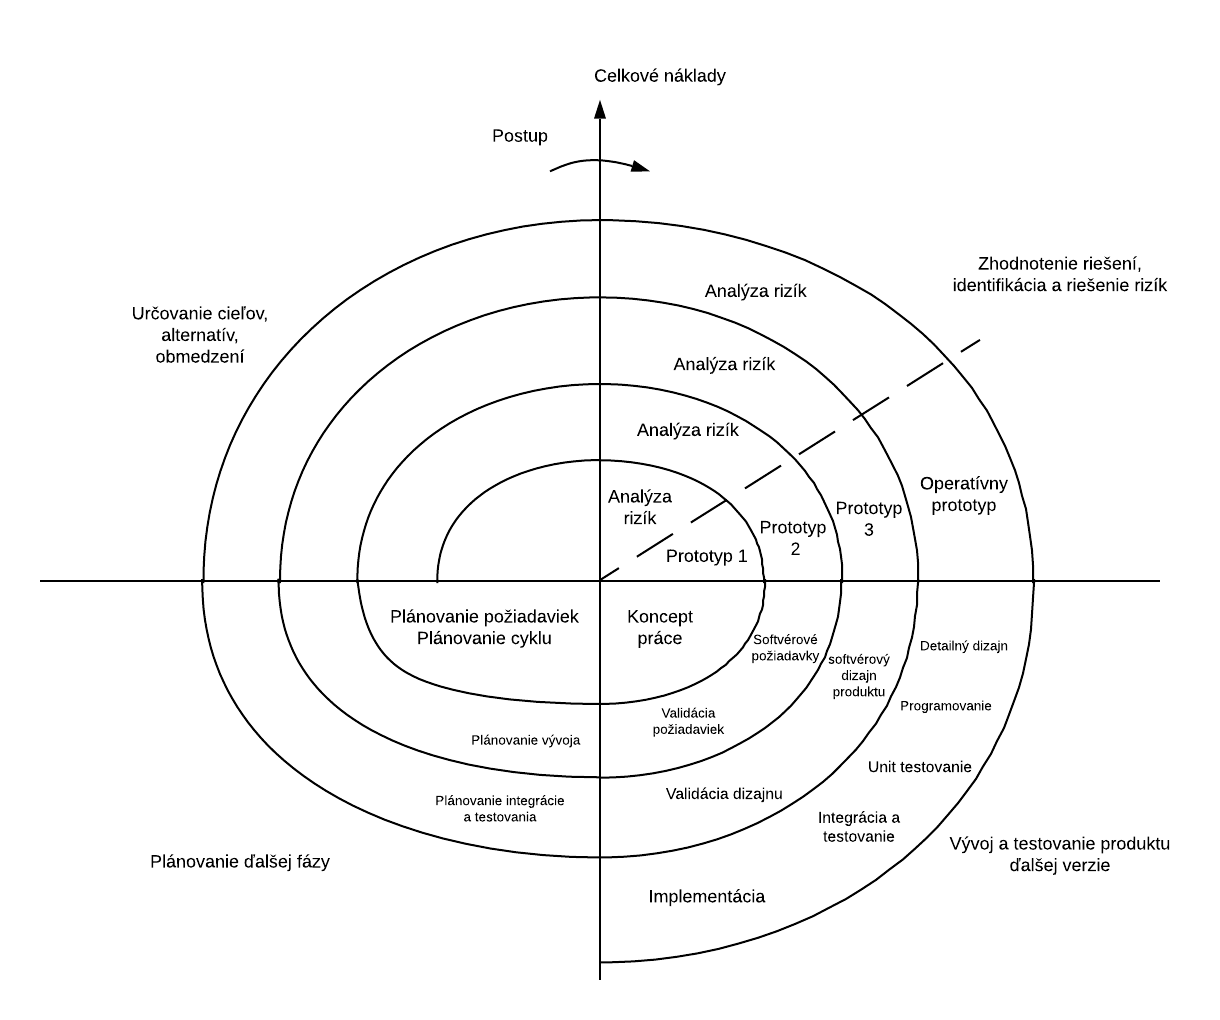
\includegraphics[width=\textwidth]{spiralModel.png}
\caption{Spiral model diagram \cite{Boehm}} 
\label{spiralDiagram}
\end{figure} 

\subsection{Riešenie rizík pomocou Spiral modelu} \label{risks:spiralModel}

Na doplnenie.

\subsection{Vznik Spiral modelu} \label{history:spiralModel}
Pred prvou definíciou Barrym Boehmom v roku 1986 sa Spiral model vyvíjal niekoľko rokov. Prvé implementácie vznikali na základe rôznych úprav Waterfall modelu aplikovaného na veľké vládne projekty. \cite{Boehm}

Na doplnenie.

\subsection{Využitie Spiral modelu} \label{usage:spiralModel}

Na doplnenie.

\subsection{Win-Win Spiral model} \label{winwin:spiralModel}

Na doplnenie.

\subsection{Problémy Spiral modelu a ich riešenia} \label{problems:spiralModel}

Na doplnenie.



\section{Záver} \label{zaver} 
Na doplnenie.



\bibliography{literatura}
\bibliographystyle{abbrv}
\end{document}
